% --------------------------------------------------------------------

\section{Introduction}

Communicating with each other using technologies, such as Bluetooth, is becoming ever more popular in the field. Both old and new emerging technologies enable us to create new ways of establishing communication between total strangers with similar interests. This thesis describes how these technologies can be used to create social interaction between strangers and therefore increase their well-being of people and their performance during sports.

Familiar strangers is a concept first introduced by the psychologist Stanley Milgram in 1972 in his essay \citep{milgram1992}. We often come across to the same strangers while doing sports, but do not interact with them. These people, that you have met frequently but never interacted with, are called familiar strangers. \citep{familiarStranger}. Familiar strangers as a concept isn't limited to sports, but targeting the research to people who have similar interests (sports) by definition makes monitoring of their behavior simpler. While social networking between strangers has been research before, this concept of social interaction between familiar strangers in sports, is new in the field.

Methods used in this paper to research this problems are:
\begin{itemize}
\item  Literature review.
\item Conducting interviews.
\item Creating a prototype application for research data.
\end{itemize}

This paper presents a prototype Android application that will log the times strangers passing by you. When you come across to a strangers enough times, the application will suggest communication with the stranger. With the prototype, you can view where and how many times you have encountered that person and what are they interested in. Interesting questions related to this prototype application are, whether users are willing to establish communication based on similar interest and similar real-life habits (sports routes and times) and also how much information users are willing to share to total strangers. Data gathered form this prototype application can later be used to verify assumptions about the users behavior and to learn new information. The prototype application takes privacy seriously and is quite conservative about sharing information. The level of privacy can later then be modified based on feedback from the users.

The application uses Bluetooth beacons to identify the strangers and log the encounters to a web server. This enables the users to interact with the strangers also outside the sports activity itself. They don't have to approach the strangers while doing sports but they can later on interact with people they have met along the way and find similar interests with. 

The interviews were composed from open-ended questions where the goal was more to find new information rather than just to validate previous assumptions. The interviews were extensive and performed only for a handful of possible end users of the application. No survey's were conducted for this thesis.

\section{Related work}

% TODO kuvaile aihekenttää yleisemmin.

This section presents related works from two perspectives: the social interaction perspective and the perspective of doing sports. The design of the prototype application relies on results from both of these perspectives.



\subsection{Social interaction}

\cite{socialAdHoc} studied ad hoc social networking with a social networking system called TWIN. In a survey conducted after the study, the method for approaching unfamiliar persons was one of the highest rated features of the system. \cite{mobileMatchmaking} conducted a survey where 90\% of the participants stated that they would use regularly a service which would help introduce nearby strangers to each other. Serendipity, the application created for their research, is a mobile match-making system which alerts users when someone with similar interests comes into proximity. The reactions to the system have been overwhelmingly positive. These results imply that systems which allow people to interact with familiar strangers are in fact desired by users.

\subsection{Sports}

Meeting strangers is only one part of the assumed benefits of the prototype application. Previous research suggests that doing sports in a group or together with a friend results in increased performance. Therefore, the findings suggest that finding strangers with similar interests and a similar level of fitness to do sports with would result in a performance increase for the user. However, finding people to do sports with can be an daunting task especially for people who have just moved to a new city or a country. It is important to make finding strangers as easy as possible with the use of modern technology without compromising the privacy of the users.

One of the concerns of creating the application is that how frequently people doing sports actually meet familiar strangers. Setting the level of passing by's before allowing users to communicate with each other affects the whole user experience of the prototype application. Research by \cite{runningNavigation} showed that distance is the key thing what joggers are thinking about while running, not about using familiar routes. However, while routes change, joggers use familiar locations more than once. They usually leave out a part or add one based on their overall feeling. The fact, that joggers reuse locations increases the probability of running into familiar strangers along the way.

\subsection{Social sports}

This section cover previous research about social sports.

\cite{joggingOverDistance} present a social prototype application called "Jogging over a Distance", where two people can jog together across the globe aided by technology. The system works so that two runners agree to jog during the same time and both agree to wear a headset and a heart rate monitor during the activity. The runners have a computer and a mobile phone with them for communicating and transmitting data among the runners. While jogging, both can hear the audio from the other runner. In addition to being able to speak with the other runner, the system uses two dimensional voice to present the relative heart rate of the other runner. This audio shows the runner whether they are running too fast or too slowly and they can adjust their speed with that information.

\cite{augmentedClimbing} presents a project called augmented climbing. The paper is about interacting with projected graphics in a climbing wall. 

This thesis focuses more on how to create and inspire social interaction rather than how the interaction can be enhanced during the sports activity. However, these  findings support the view that social and augmented technology can increase performance in sports and turn a hard job into a more social play.

\subsection{Bluetooth beacons}

% TODO Add footnote to beacon models and source for bluetooth standards.

The prototype application created for this thesis uses Bluetooth beacons. Most famous commercial beacons currently are iBeacons from Apple\footnote{\url{https://developer.apple.com/ibeacon/}} and Estimote\footnote{\url{http://estimote.com/}} beacons. The beacons implement a protocol called Bluetooth low energy (BLE), which is a part of the Bluetooth 4.0 standard defined by \cite{bluetooth}. In the prototype application created for this thesis, the beacons are used to log encounters with strangers. The beacons are constantly broadcasting a message and the Android application can detect beacons while doing sports. The beacons' MAC address are used to identify the beacons uniquely. Each user is able to register one beacon for their use in the application so storing the encounters is rather easy.

The BLE protocol stack is divided into two parts, the controller and the host.

\citep{bluetoothOverview} presents findings that Bluetooth low energy consumes a lot of battery power which can be reduced by requesting data less frequently from the BLE device. This needs to be taken into account while using and developing the prototype application in order to make it as efficient as possible.

Some of the latest phones in the market are now also able to act as the peripheral role. Therefore, this application could already be done without the need of separate Bluetooth beacons. However, there are only a handful of devices that are capable of this, which results in that this prototype application would be hard to test with a big group because the phone models are still rare.

\section{Interviews}

This section describes the methods used for the interviews and the results gained from them. All interviews are anonymous and only basic demographic information about age and sex was gathered from the participants.

\subsection{Method for the interviews}

The interviews consist multiple open-ended questions. The goal is to find out information about how people behave while doing sports and what are their thoughts about the prototype application. The main questions for the interview are are located in appendix \ref{sec:app1_1}.

The questions aren't meant to be strict but just as a guideline for the discussion. If new interesting discussions emerge while interviewing, the idea is to go forward with them without thinking too much about the guideline.

The goal of the interviews was to do explorative research about possible directions for the design of the prototype application.

\subsection{Results}

In total, three people were interviewed for this thesis. A few demographic questions were included in the interviews. Two of the participants were female and one was  a male. One of the participants did sports four to five times a week, one two to three times a week and one did sports rarely (less than weekly). Their sports activities were gym, various group exercises (e.g. spinning), martial arts and jogging.

One of the participants was very goal oriented in their sports activities, others were doing spots just for getting a good feeling out of it. All of them carried devices for music during sports. Therefore, using the kind of a prototype application done for this thesis wouldn't require a change in their current behavior. Most of them did sports alone, sometimes together with friends. Friends that they did sports with, were mostly old friends from school. One of them got to know strangers that they frequently met at the gym and later started working out together.

Doing sports together with other people and alone had different effects to their motivation. One of the participants said that they didn't feel any difference in motivation when doing sports with or without friends. Others felt some differences.

\begin{quotation}
\it I might have a good motivation with or without friends. In a group settings, others are supporting me, which might make me achieve higher goals than I thought was possible. However, it might also end up so that we are just chatting without actually getting anything done. If I am working by myself, I try to gain motivation with some external factors (e.g. music or watching inspiring videos).
\end{quotation}

Privacy was a concern among the participants related to this prototype application. The initial thought for one of them was that strangers would start to stalk them using this kind of an application. One other participant quickly dismissed the idea by saying that of course showing any personal information should be voluntary. Some concerns were also brought up about criminals, such as pedofiles using this application for criminal activities. The same participant dismissed this idea also by saying that the application has no role in that situation if the people are actually meeting each other in real life all the time. However, initial reactions about privacy are important when designing an application that feels safe to use.

When asked about what they would be willing to share to strangers, the answers differed. One of them felt quite easy about sharing plenty of information.

\begin{quotation}
\it I would maybe be willing to share some open text related to my interests, my profile picture, my sex, my first name and maybe my email address. If it were a dating service and I would be actively searching for a partner, I would be willing to share more information.
\end{quotation}

One of the participant felt anxious about sharing a profile picture. One felt that profile pictures weren't necessary if the search is for a person to do sports with. Overall, they felt that the most important aspect would be to share an open field where one could describe what they are interested in and perhaps write about the kinds of people they are looking to do sports with. In addition, they felt that being optionally able to select a sex for the familiar strangers would be a good thing. They felt that most people would probably want to select a gender for people to interact and to do sports with.

\begin{quotation}
\it If I am looking for someone to spot me at the gym, I don't want it to be someone who weights 20kg or if a woman is searching for a yoga partner, they might feel more comfortable if the partner is female as well.
\end{quotation}

When asked, if they were willing to use the application to meet strangers to do sports with, the participants were hesitant.

\begin{quotation}
\it Possibly yes, if it were possible to find good people to work out with.
\end{quotation}

One of the participants said that they would be willing to use it if they were single, not otherwise. One of them said that they wouldn't use the application themselves but understand if others would want to.

Interviews of three people aren't enough to draw exact conclusions about whether this kind of social interaction enhanced by an application is something people are looking for. However, this interview yield some good directions for the application on what makes people anxious and how far boundaries can be pushed while maintaining an overall safe feeling for the application.


\section{Design}

The prototype application's main goal is to allow people to connect with familiar strangers and find people to do sports with. Of course the application can be used for other purposes than just sports, but it is mainly designed for that challenge. It will be interesting to see whether it is used for just random encounters instead of encounters with a specific goal in mind (sports in this case). The designed process of meeting a familiar strangers and connecting with them can be divided into a few steps.

\begin{itemize}
	\item Pass by the person enough times
	\item View information about the person and their interests when the application suggests communication.
	\item Message the stranger and see if they share common goals.
	\item View their real-life information after both agree to do it and start doing sports with them.
\end{itemize}

This prototype application is a mix of remote and social interaction among people assisted with technology. Users are able to chat with familiar strangers remotely but real life proximity is required to start these conversations. The aim is to push the boundaries of how social interaction is initialized among strangers. Shared common interests are often the starters for social interaction among strangers and the application tries to highlight these common interests and make the process as smooth as possible.

\subsection{Passing by}

Using Bluetooth beacons, the application will log every person that passes by. Only one of the users have to have their mobile phone with them, since all the encounters are stored in the server. The hard part of this section is to select the amount of pass by's that initialize communication between the users. The initial default value is three times. This can easily be adjusted from the server later so no additional application releases need to be made. Three times will most likely be too low when the amount of users for the application grow. If a larger study is done later to validate the users behaviors, the amount should be increased. The users are also able to select the amount themselves before other users are able to approach them with messages. The conducted interview suggests that people would be interested to see the public interests of strangers even with low encounters.

The users are also able to select few requirements for the encounters, such as sex of the stranger. Therefore, if the user is searching for male joggers, no females will be suggested for interaction.

\begin{figure}[htb]
	\begin{center}
		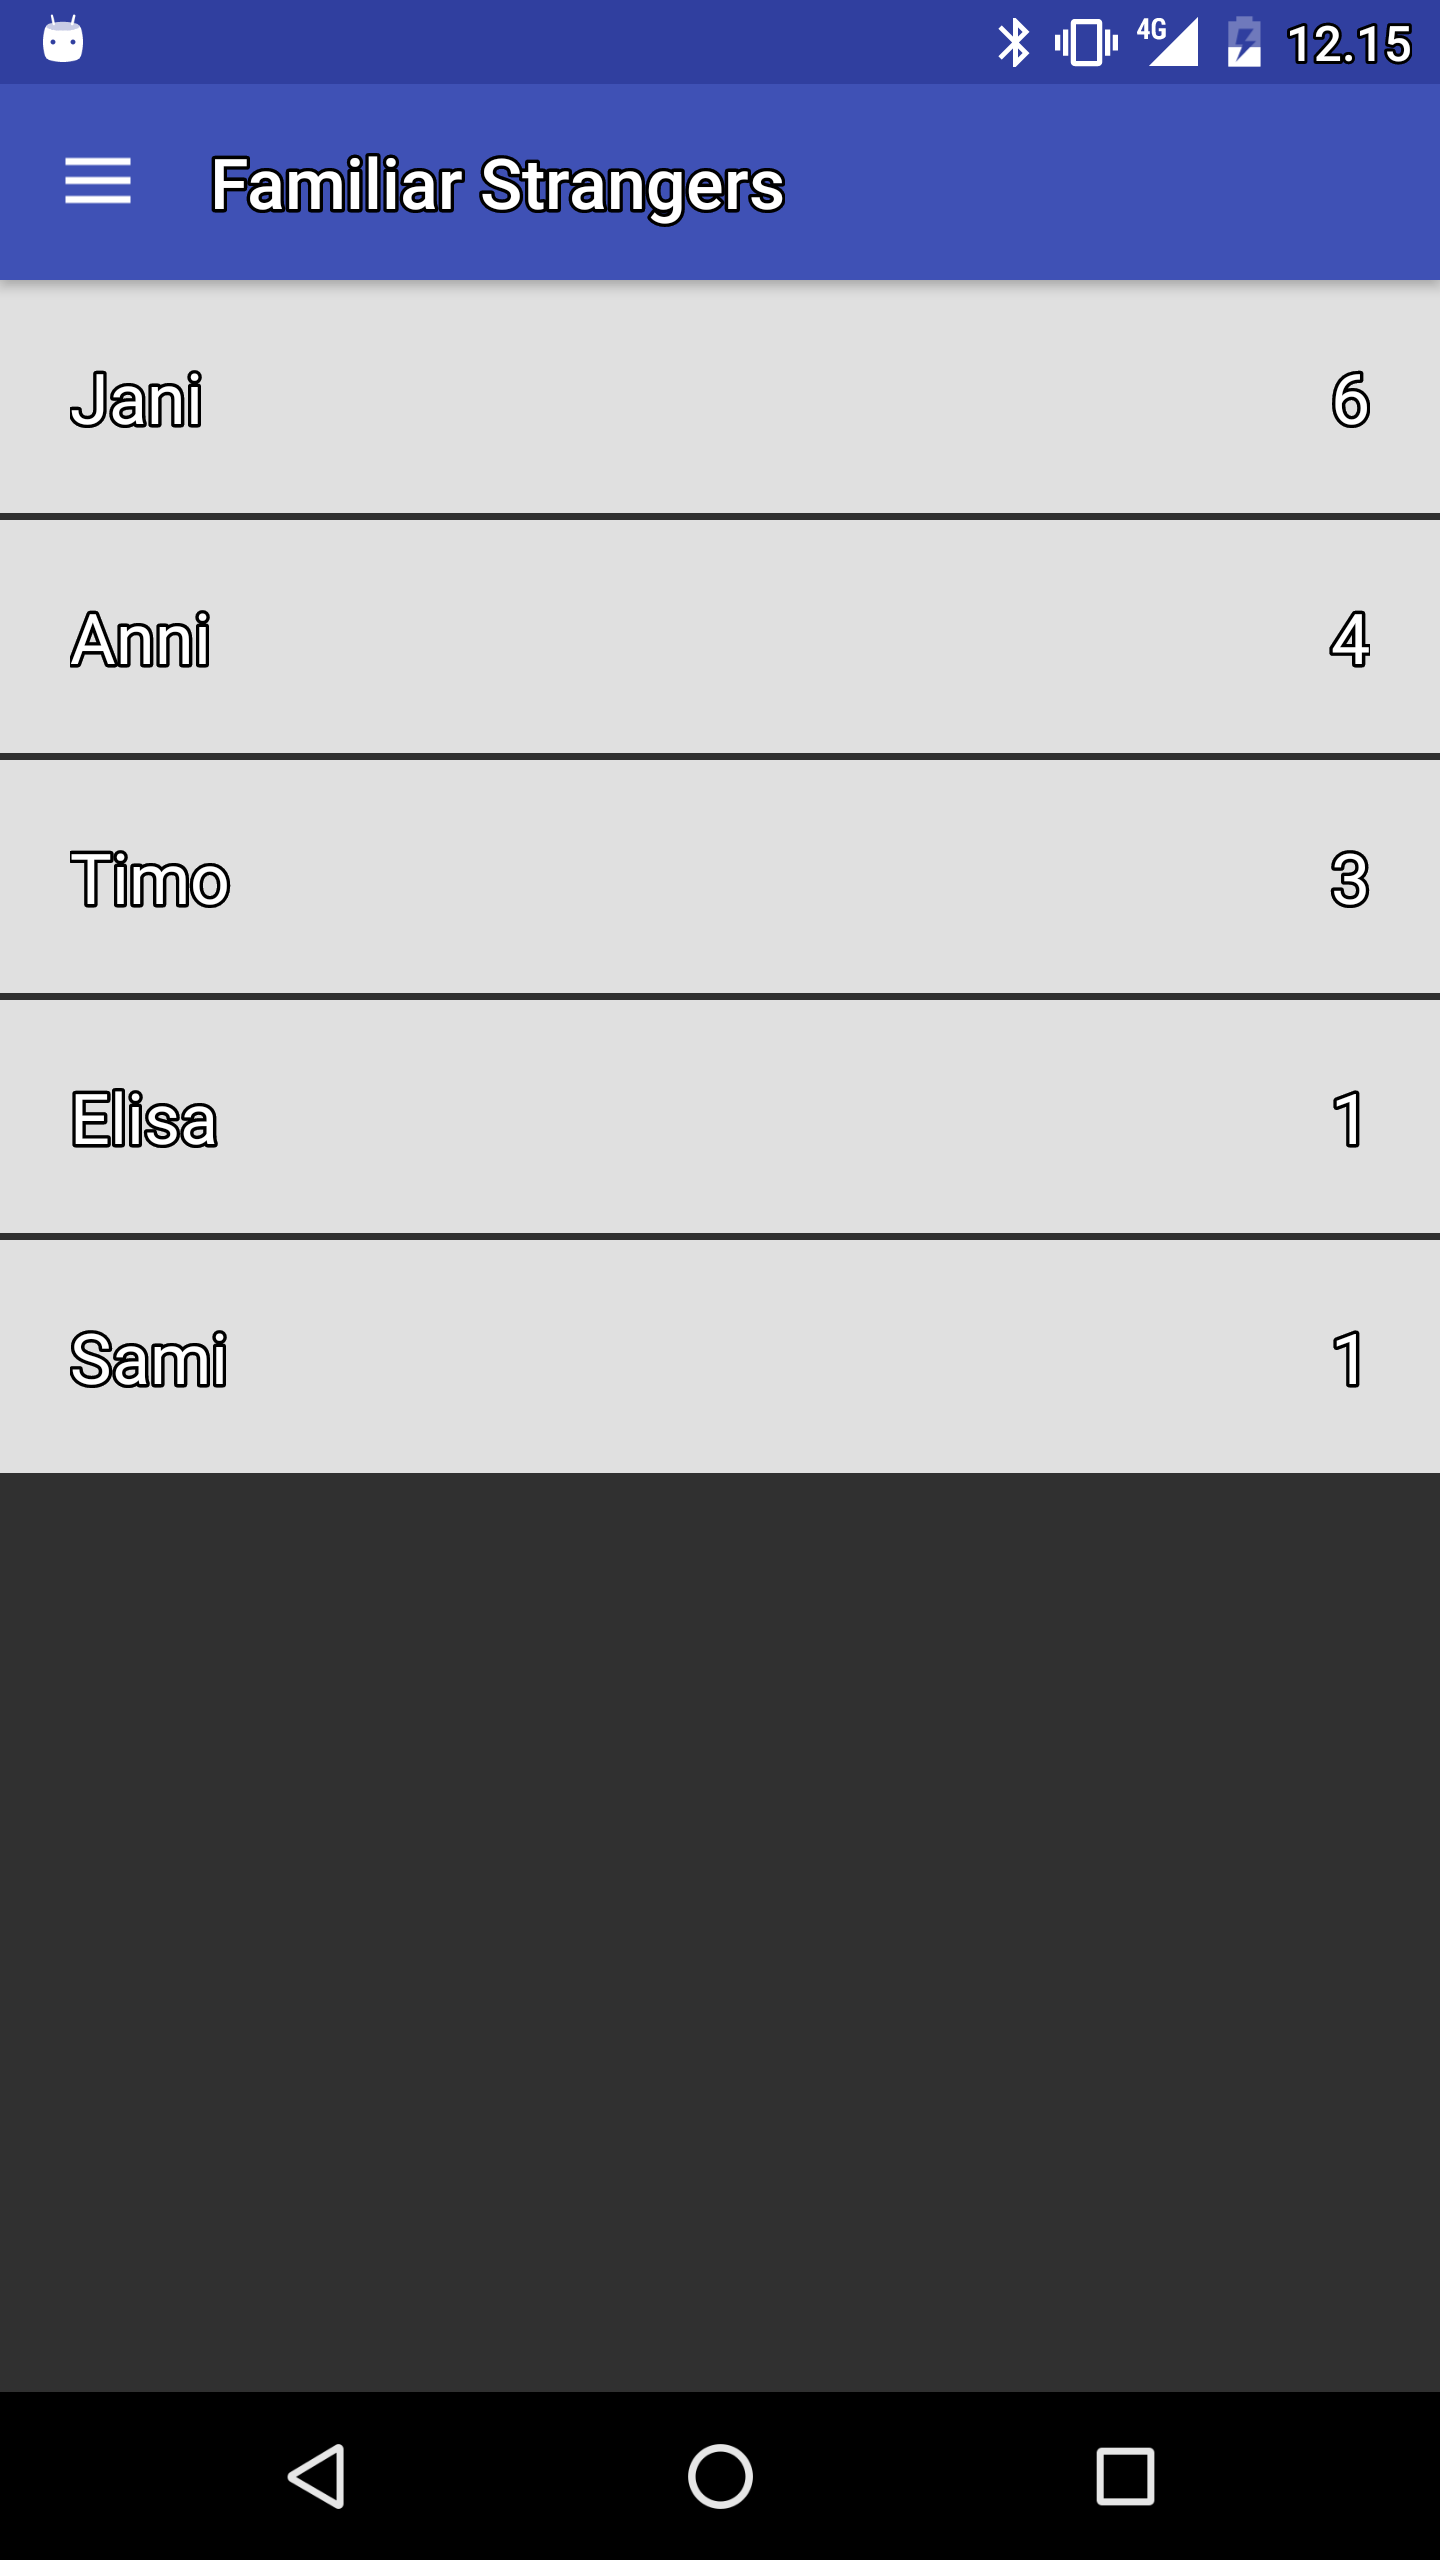
\includegraphics[width=0.4\textwidth]{encounters.png}
		\caption{A list of encounters (name and how many times)}	
	\end{center}
\end{figure}

The user is able to view how many people they have come encountered from a list in the application. The list shows the user with an unique identification (not their real name) and also the times they have come across each other. If the strangers has enabled other information to be public, such as a profile picture, those will be displayed at this point as well.

The logging can be turned on and off whenever the user feels like it. The reason could be that the user is in a place where they do not want to encounter anyone or have a record of the location stored in the application or if they want to save battery by closing every Bluetooth connection. It will also be interesting to see whether people will keep it on always, or just during the activities they want to perform with other people, such as sports.

\subsection{Approaching the stranger}

After the user has encountered a familiar stranger enough times, the application will suggest communication between both parties. The user will see the other persons public interest that they have filled while registering to the application and also display on a map where they have encountered each other. As a result of the interviews conducted for this thesis, I decided not to include any other visible data for other users at this point. Based on the literature review of this thesis and the interviews, displaying this kind of information publicly to the users shouldn't be a problem for the majority of users. However, the user can optionally display more information, such as a profile picture already at this stage.

The interaction can stay anonymous as long as the users want to. It's possible to send messages to each other just to ask what they are interested in and see if both of them would be interested in doing sports together. The chat is meant for users to verify similar interests and goals before getting to know each other better. If the interests and goals do not match, either user can ignore the other person and they will not be in any kind of interaction via the application ever again.

\subsection{Revealing identity}

At some point, it is necessary to reveal real life information in order to initialize social interaction among the two strangers. The real life information should be revealed only after both parties feel entirely comfortable with the idea. There, in this prototype application, it is possible for the user to request real life information from the other person and only after both parties agree to reveal information will anything be revealed. The information can be revealed one piece at a time or all at once. After revealing information, it is possible for both of them to start doing sports together or find other meaningful things to do in life. Most likely the two will not continue chatting via this application after this point, but it is possible to do so. A record of their communication is left on the app, and it will not log any encounters from the other person anymore at this point. Until real life information is accepted, the application will still log encounters from the person and view them in the list of encounters unless the user removes them manually.

It is interesting too see whether revealing real life information one at a time create a more comfortable environment or will everyone just reveal all of the information at once. I was unable to find any references to a similar method used in another application. Therefore, this kind of a mutual information revealing piece by piece seems to be quite new in the field.

\section{Prototype implementation}

The created prototype is an Android\footnote{\url{https://www.android.com/}} application. The programming language selected for the application is Kotlin\footnote{\url{https://kotlinlang.org/}}. Kotlin helped to reduce the amount of bugs during the creation process and proved to be a very fast programming language for d	keveloping Android applications. In addition to Kotlin, Anko\footnote{\url{https://github.com/Kotlin/anko}}; a view library created by JetBrains\footnote{\url{https://www.jetbrains.com/}}; was also used for the application. Using Anko reduced the amount of time going to creating basic views, e.g. for the login and registering views.

\subsection{Architecture}

\begin{figure}[htb]
	\begin{center}
		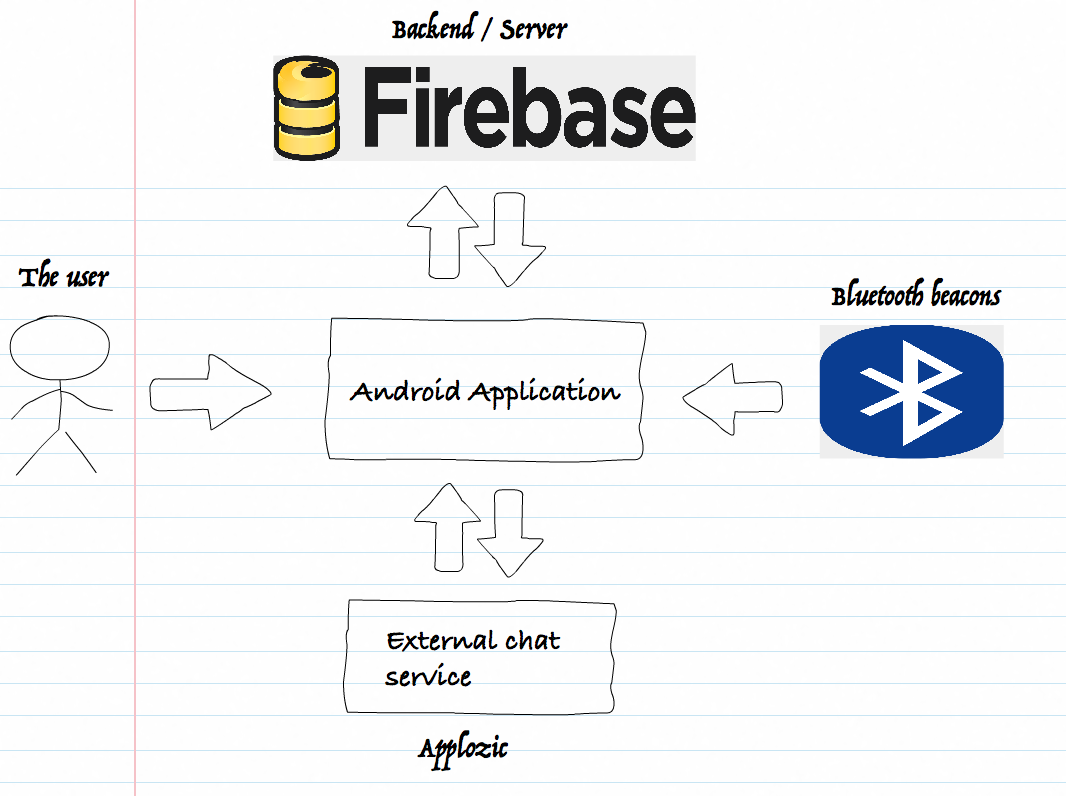
\includegraphics[width=0.8\textwidth]{fs_architecture.png}
		\caption{The application architecture.}	
	\end{center}
\end{figure}

The application is divided into a client (the Android application) and a backend (server). The backend is built with Firebase\footnote{\url{https://www.firebase.com/}}, which is a tool for creating fast backends using nothing but JSON\footnote{Javascript Object Notation} objects. The user authenticates to the backend, so that we get unique users ID's that aren't locked into a single device in the application's lifetime. In addition to Firebase, the application uses an external chat service for the messaging feature.

The application uses Firebase's authentication features for the authentication. A combination of email and password is currently used. However, it is easy to add third party login systems, such as Facebook\footnote{\url{https://www.facebook.com/}} and Google\footnote{\url{https://www.google.com}} for the authentication.

The application uses a background service to run the logging of encounters among the users in a separate thread. The background service detects the join and exit events of Bluetooth beacons and based on those events, sends the server information about the encounters. This background service will stay running even though the user is not currently actively using the application. Monitoring the events for Bluetooth beacons drains extra battery from the phones. It remains to see, if the application uses too much battery so that the users will uninstall the application.

Push notifications are not at the moment handled by a real-time push notification server. The application polls the Firebase server periodically and sees if there are any changes available. This will hopefully be improved in the future.

\subsection{Description of functionality}

\begin{figure}[htb]
	\begin{center}
		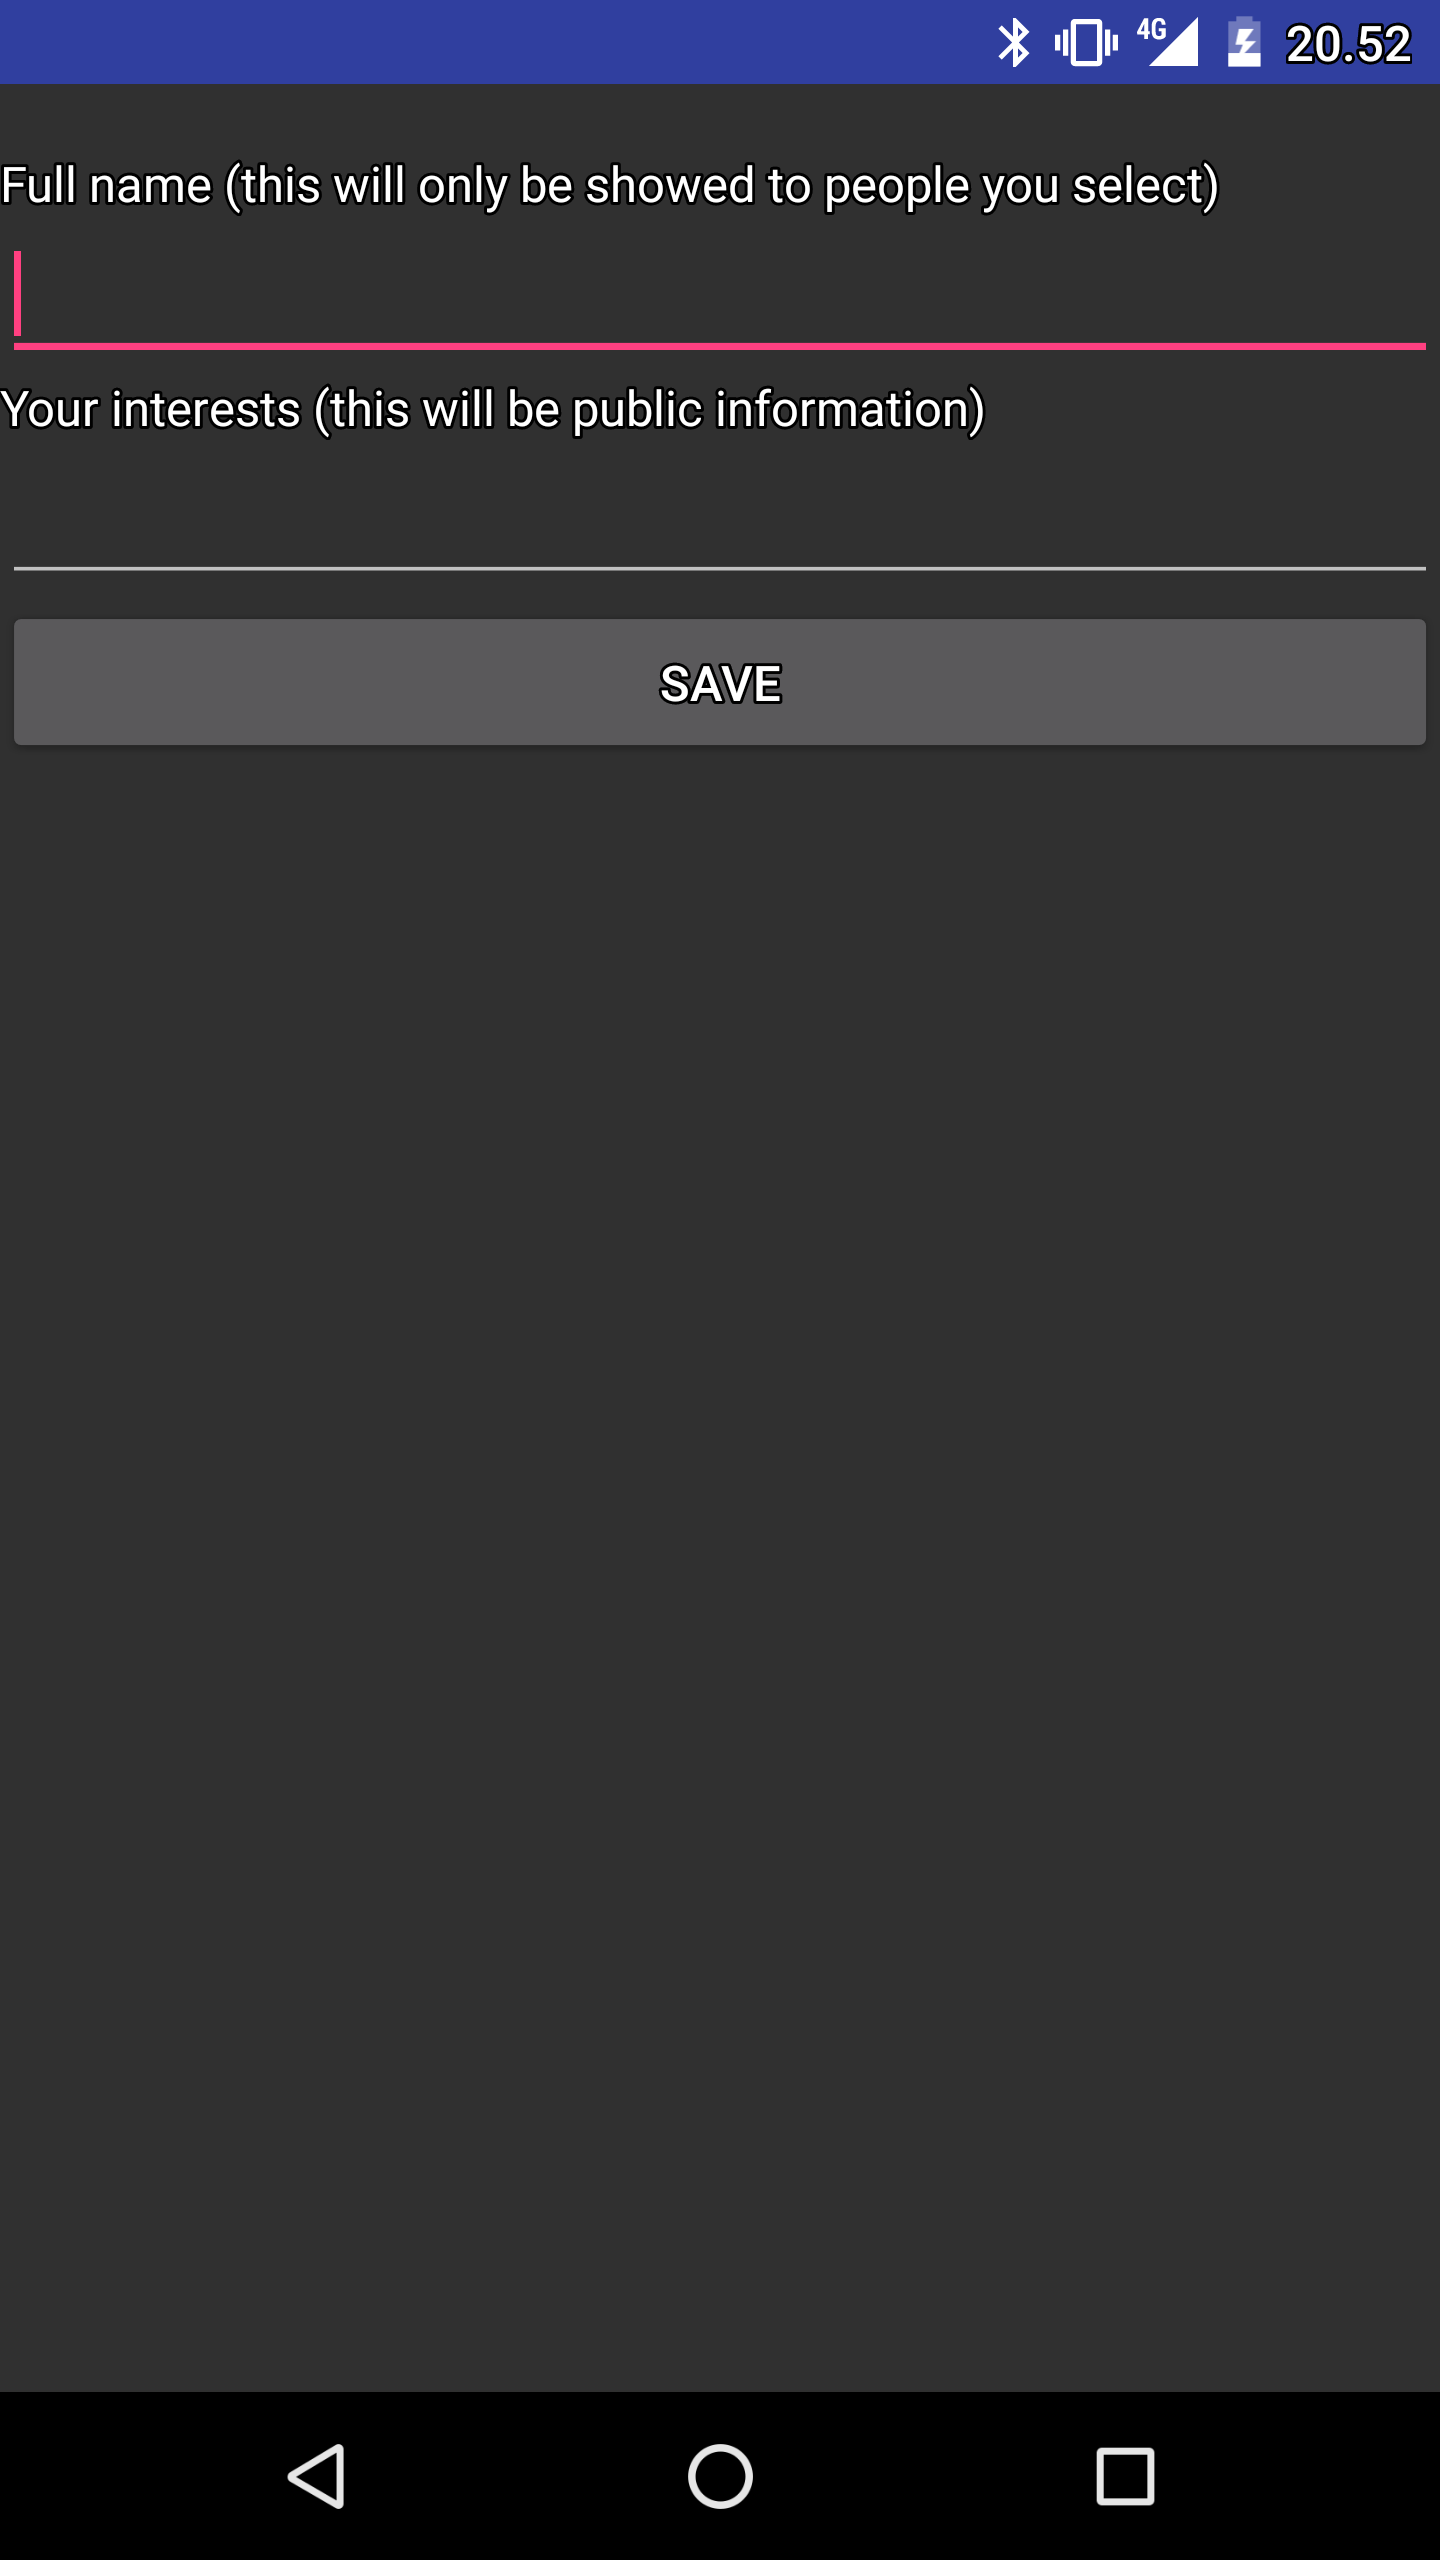
\includegraphics[width=0.4\textwidth]{fs_onboarding.png}
		\caption{Filling personal information.}
	\end{center}
\end{figure}

When starting the application for the first time an onboarding process wil begin for the user. The user is required to register for the application. They can also just log in with an existing account so using the application isn't tied to a single device. After that the user is required to fill their profile information. The fields required for this are their name and public interests. After completing this stage of the onboarding the user is required to register a beacon for their use. At this point the application will detect every beacon nearby and show them in a list as seen in figure X. This completes the onboarding process and the user is now free to use the application.

\subsection{Using the prototype}

The application is open sourced with the Apache 2.0 license\footnote{\url{http://www.apache.org/licenses/LICENSE-2.0}}. Therefore, anyone is free to take it into use, modify it or even make money out of it. A few steps are needed before the application can be taken into use by someone. First of all, the application uses Firebase as the backend service. Therefore, a Firebase account and an application created with it is required for using this application. The data structure for the JSON objects used in Firebase is described in the appliation's source code, so developing a custom backend for the application is entirely possible and quite fast to do.

\section{Discussion}

This section analyses the results that the study produced and what should be done in the future related to the created prototype application and about researching the social interactions of familiar strangers.

\subsection{Results of the study}

The conducted interviews presented multiple interesting points of views. However, as the amount of interviews is so low, it is not possible to draw general conclusions about the behavior models of users. The results served their purpose in giving general direction to the prototype application's design process and therefore resulted in very valuable information for this study.

The prototype application is functional and it its possible to use it for further research. The application is also open source so it's easy to take into use in any research facilities across the globe.

\subsection{Future work}

A larger study should be conducted to validate the behavior models and assumptions that were generated by the conducted interviews. In addition to researching the behavior models of doing social interaction among familiar strangers, the prototype application should be used for more and bigger research.

Doing research with this application requires quite a big user study in order to create an environment where actual encounters with strangers will happen. Unfortunately no such large study has been done for this thesis, but as the application is licensed with an open source license, hopefully such study will see the light of day sometime in the near future. The future research done by this application should also take into account different kinds of sports and the 	behavior among them.

Some additional functionality is planned for the application. The proposed features are listed in the GitHub page of the application. At this point it is unclear whether those features will be implemented, but they are there for anyone to take. Modifications to the code and complete new features are by all means welcome.

% --------------------------------------------------------------------
